\documentclass[runningheads]{llncs}
\usepackage[T1]{fontenc}
\usepackage{graphicx}
\usepackage{amsmath}
\usepackage{booktabs}
\usepackage{xcolor}
\usepackage[hidelinks]{hyperref}

\begin{document}

\title{Receptive Field, Not Attention: What Improves Lightweight Violence Detection}
\titlerunning{Receptive Field, Not Attention}

\author{Nguyen Huu Hoang \and Ngo Thanh Trung}
\authorrunning{N. H. Hoang and N. T. Trung}
\institute{School of Information and Communications Technology,\\
Hanoi University of Science and Technology, Hanoi, Vietnam\\
\email{hoang.nh225972@sis.hust.edu.vn}}

\maketitle

\begin{abstract}
Violence detection runs on every camera of a surveillance installation, so
the deployed model has to be small, and the literature reports steady gains
from cheap modules added to small video networks. We measure which of these
gains hold up. On RWF-2000, Hockey Fights and RLVS we remove duplicated
clips, keep clips of the same scene in one fold, take every decision on
out-of-fold predictions and score each test split once. Three results
follow. First, the person-detection crop that this line of work applies
before the network costs 2.97 out-of-fold points ($p=0.0002$); decoding and
resizing the video, with no detector, is both the most accurate and the
cheapest pipeline. Second, enlarging the channel-wise kernels of every
stage of X3D-M to $5\times5$, trained as a zero-initialised ring that fuses
into one kernel for inference, adds 2.63 test points over three seeds,
while the same widening in the first two stages only adds 0.75. Third, a
motion-attention gate adds nothing, and the same gate fed an all-zero
motion map performs as well. Averaging the weights of the four fold models
that the protocol trains anyway gives one model as accurate as their
ensemble. The final detector reaches 91.6\% on RWF-2000 with 3.3M
parameters and 5.9 GFLOPs per clip.

\keywords{Violence detection \and Efficient 3D CNN \and Receptive field
\and Structural reparameterisation \and Evaluation protocol.}
\end{abstract}

%======================================================================
\section{Introduction}

Surveillance cameras are installed at a scale that human operators cannot
watch: an estimated 770 million were in use by 2019~\cite{cnbc2019}, and an
observer's ability to notice rare events declines within twenty minutes of
continuous monitoring~\cite{mackworth1948}. Automatic violence detection
flags the few streams that need attention. Because it runs on every camera,
the model must be cheap. The most accurate models on
RWF-2000~\cite{rwf2000} are far from that budget: CUE-Net~\cite{cuenet}
reports 94.0\% with 354M parameters, and video transformers report
91.8--92.4\% with 67M to 305M parameters~\cite{videomae,mixvit}. A second
line of work~\cite{rwf2000,sepconvlstm,mdcn,biltma} stays within a few
GFLOPs and reports 87--90\%, usually by adding a module to a compact
backbone: a motion branch, an attention block, or a wider kernel.

This paper asks how much such additions contribute once they are measured
carefully. We study two of them on X3D-M~\cite{x3d}: a Motion Attention
gate that rescales features with a multi-scale frame difference, and a
reparameterised wide kernel that enlarges the channel-wise convolutions to
$5\times5$ and fuses away at inference. The benchmarks do not make such a
measurement easy. RWF-2000 has no validation split, so checkpoints are
often chosen on the test split; nine of its training clips are copies of
test clips; and single training runs are noisy enough to produce
significant-looking differences by chance. We therefore remove duplicates,
keep same-scene clips in one fold, take every decision on four-fold
out-of-fold (OOF) predictions, repeat the key comparisons over three seeds,
and score each test split once.

Under that protocol the two modules behave very differently. Motion
Attention adds nothing, and a control that feeds the gate an all-zero
motion map does as well as the real one, so the gate does not use the
signal it is built on. The wide kernel helps, but only once it is applied
to all four stages rather than the first two: most of its gain comes from
the late stages, where the feature maps are small and a $5\times5$ kernel
covers much of the scene. The largest effect, however, lies outside the
network. The pipeline that the task inherits detects people and crops the
video to them before the network sees it. Rebuilding RWF-2000 from the raw
videos seven times shows that this crop costs about three points, and that
the best pipeline has no detector in it. Our contributions are:

\begin{itemize}
  \item A controlled study of the input pipeline, showing that the
    person-box crop costs 2.97 OOF points and that the most accurate
    pipeline is also the cheapest (Sect.~\ref{sec:pipeline}).
  \item A study of where and how far to widen the kernels of a compact 3D
    network, with a gain of 2.63 test points that holds over three seeds
    and fuses away at inference (Sect.~\ref{sec:kernels}).
  \item A negative result for motion gating with the control that explains
    it (Sect.~\ref{sec:ma-result}).
  \item A uniform soup of the fold models, which turns the models trained
    for an honest estimate into one deployable model as accurate as their
    ensemble, replicated on nine experiments (Sect.~\ref{sec:soup-result}).
\end{itemize}

%======================================================================
\section{Related Work}

\textbf{Violence detection.} Early methods encoded motion with dense
trajectories~\cite{idt}, flow magnitude~\cite{vif} or
acceleration~\cite{hockey}. Two-stream networks~\cite{twostream} add
optical flow, often at a higher cost than the network itself; 3D
convolutional networks~\cite{c3d,i3d,slowfast,x3d} learn from RGB alone,
and video transformers~\cite{timesformer,videoswin} rely on large-scale
pre-training. On RWF-2000, the Flow Gated Network~\cite{rwf2000} reaches
87.25\%, SepConvLSTM~\cite{sepconvlstm} 89.75\%, a two-stream
multi-dimensional network~\cite{mdcn} 89.70\% below one million
parameters, and an EfficientNet with bidirectional motion attention and
temporal shift~\cite{biltma} 90.25\%. CUE-Net~\cite{cuenet} and our
earlier configuration first detect people and crop the frame to them. Most
of these works report accuracy on the official test split without stating how
the checkpoint was chosen.

\textbf{Efficient backbones and large kernels.} X3D~\cite{x3d} expands a
small network one axis at a time; X3D-M reaches 76.0\% on Kinetics-400 with
3.8M parameters. Structural reparameterisation~\cite{repvgg,acnet} trains
extra branches and fuses them into one kernel for inference, and
RepLKNet~\cite{replknet,unireplknet} uses it to train very large kernels in
2D networks. We use the same principle on the channel-wise 3D kernels of a
pre-trained video network, where the question is less how large a kernel
can be than where a modest enlargement pays off.

\textbf{Gating and weight averaging.} Multiplicative gates such as
squeeze-and-excitation~\cite{se} re-weight features with a learned signal.
Model soups~\cite{soup} average the weights of models fine-tuned from the
same initialisation and often match their ensemble; we apply the idea to
the fold models of a cross-validation protocol.

%======================================================================
\section{Method}
\label{sec:method}

\textbf{Backbone.} A clip is an RGB tensor of 16 frames at
$224\times224$. X3D-M~\cite{x3d}, pre-trained on
Kinetics-400~\cite{kinetics}, has a stem and four stages (Res2--Res5 with
3, 5, 11 and 7 blocks) whose outputs are $56^2$, $28^2$, $14^2$ and $7^2$
at full temporal resolution. Each block holds a $3\times3\times3$
channel-wise convolution between two $1\times1\times1$ projections. The head
pools globally and ends in a new two-way classifier.

\textbf{Wide-kernel reparameterisation.} Let $W_{\text{base}}$ be the
pre-trained $3\times3\times3$ channel-wise kernel of a block. It is replaced
by
\begin{equation}
  W_{\text{eff}} = \mathcal{P}(W_{\text{base}}) + M_{\text{ring}} \odot \Delta ,
  \label{eq:rep}
\end{equation}
where $\mathcal{P}$ zero-pads the spatial dimensions to $5\times5$,
$\Delta$ is initialised to zero and $M_{\text{ring}}$ is one on the 16 outer
positions of each $5\times5$ slice. At initialisation the network is
exactly the pre-trained one. Convolution is linear in its kernel, so after
training the two terms are summed into one $3\times5\times5$ kernel and
inference runs a plain X3D with slightly larger kernels; the fused and
unfused networks agree to $4\times10^{-7}$ in output probability. Keeping
$\Delta$ as its own tensor has two consequences. It is trained at the
learning rate of new parameters rather than that of the backbone, and it can
be trained in a stage whose pre-trained weights stay frozen: the recipe
below keeps Res4 frozen, and the ring still widens it. We apply the ring to
every block of every stage (Fig.~\ref{fig:kernel}), which adds 0.29M
parameters (0.46M during training) and 1.19 GFLOPs.

\begin{figure}[t]
\centering
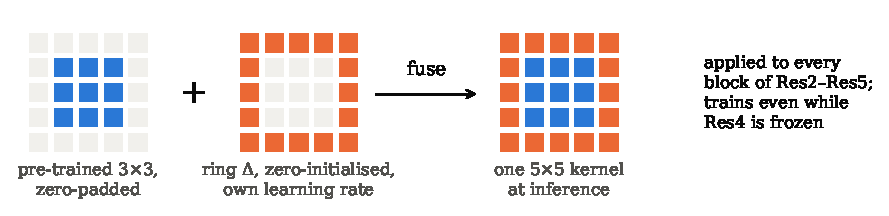
\includegraphics[width=\linewidth]{fig_kernel}
\caption{The reparameterised wide kernel. The pre-trained $3\times3$ kernel
is zero-padded to $5\times5$ and a zero-initialised ring $\Delta$ is added
(Eq.~\ref{eq:rep}); after training the two are summed into one kernel, so
the deployed network is a plain X3D with $5\times5$ channel-wise kernels.}
\label{fig:kernel}
\end{figure}

\textbf{Motion Attention.} The module we compare against computes a motion
map $m_t=\min(\max(d^{(1)}_t, d^{(2)}_t),\delta)/\delta$ from the
channel-averaged absolute frame differences at steps 1 and 2
($\delta=0.2$), turns it into four temporal modes with a learned temporal
convolution, and maps them to a gain on the Res4 features,
\begin{equation}
  Y = F \odot (1+G), \qquad G = \tanh\!\left(W_2\,\mathrm{ReLU}(W_1 \tilde{M}) + b_2\right),
\end{equation}
with $W_2$ initialised near zero, so the module starts as an identity. It
varies the gain over channels, time and position and has 2{,}508
parameters.

\textbf{Fold soup.} The protocol of Sect.~\ref{sec:protocol} trains four
models, one per fold, from the same pre-trained weights. Instead of
retraining on the whole training split or deploying their four-model
ensemble, we average their weights uniformly into one network. The recipe
is fixed in advance, every fold with equal weight, so scoring it on the
test split involves no selection.

\textbf{Training.} In a probe phase of four epochs at $10^{-3}$ only the
classifier and the new modules train. In the fine-tuning phase Res2, Res3,
Res5 and the head train at $5\times10^{-5}$ and new parameters, including
the rings, at $5\times10^{-4}$; the stem and Res4 stay frozen. We use
AdamW~\cite{adamw} with weight decay $5\times10^{-4}$, a cosine schedule,
label smoothing~\cite{labelsmoothing} of 0.1, CutMix~\cite{cutmix} on half
of the batches, batches of 12 clips, 48 epochs with patience 16 and an
exponential moving average of the weights. Augmentation draws one set of
parameters per clip (photometric changes, flip, crop of 70--100\%, rotation
of $\pm10^\circ$, playback speed) and applies it to every frame. At test
time 16 frames are spread evenly over the clip, one view.

%======================================================================
\section{Evaluation Protocol}
\label{sec:protocol}

\textbf{Datasets.} RWF-2000~\cite{rwf2000} has 2{,}000 five-second clips of
fights and non-violent activity, mostly from surveillance cameras, split
into 1{,}600 training and 400 test clips. Hockey Fights~\cite{hockey} has
1{,}000 clips from ice-hockey games and RLVS~\cite{rlvs} 2{,}000 clips of
street fights and everyday activities; neither has an official split, so we
draw 20\% of each as a test set by whole same-scene groups. Every clip is
stored as 64 frames.

\textbf{Duplicate audit.} Each clip is described by four evenly spaced
frames, converted to grey, pooled to $16\times16$ and standardised; two
clips are compared by the cosine similarity of their descriptors. Pairs
above 0.99 are treated as copies and pairs above 0.9 as the same scene. In
RWF-2000, nine training clips are copies of test clips; with the second
copies of duplicated training pairs, we remove 16 training clips, leaving
1{,}584 in 1{,}579 same-scene groups. Hockey Fights and RLVS keep 797 and
1{,}588 training clips after the same audit.

\textbf{Decisions and statistics.} None of the benchmarks has a validation
split. We divide each training split into four folds, stratified by class
and never separating a same-scene group, and keep the checkpoint with the
best validation F1 in each. The four validation sets cover every training
clip once, which gives one OOF prediction per clip; every choice in this
paper is made on these predictions, and the test split is scored once.
Unless stated otherwise, test accuracy is the mean over the four fold
models, each trained on 75\% of the training clips. Paired comparisons use
the exact McNemar test~\cite{mcnemar} and 95\% bootstrap intervals over
clips~\cite{bootstrap}. On the 1{,}584 OOF clips of RWF-2000 the half-width
of this interval is about 1.1 points; on its 400 test clips one point is
four clips, which is why the central comparisons use three seeds.

%======================================================================
\section{Experiments}
\label{sec:results}

\subsection{The input pipeline}
\label{sec:pipeline}

The pipeline of our earlier configuration detects people with
YOLOv8n~\cite{yolov8} on 12 frames per clip, clusters the box centres with
DBSCAN~\cite{dbscan}, crops every frame to the largest cluster with a 20\%
margin, equalises contrast with CLAHE~\cite{clahe} and resizes to
$224\times224$. We rebuilt RWF-2000 from the raw videos seven times,
changing one step at a time, and trained the same network (X3D-M with
Motion Attention and wide kernels in Res2--Res3) with the same recipe on the
same folds (Table~\ref{tab:pipeline}).

\begin{table}[t]
\centering
\caption{RWF-2000 rebuilt from the raw videos, one preprocessing step at a
time; same network, recipe and folds, seed 0. $\Delta$ and $p$ are against
the original pipeline (row 6), exact McNemar on the OOF predictions.}
\label{tab:pipeline}
\setlength{\tabcolsep}{5pt}
\begin{tabular}{llcccrc}
\toprule
Crop & Contrast & Resize & OOF & Test & $\Delta$ OOF & $p$ \\
\midrule
none              & CLAHE & stretch & \textbf{92.55} & 89.50 & $+2.97$ & 0.0002 \\
none              & --    & stretch & 92.42 & 89.75 & $+2.84$ & 0.0003 \\
none              & CLAHE & pad     & 92.36 & 88.75 & $+2.78$ & 0.0008 \\
$\geq$ half frame & CLAHE & stretch & 91.98 & 89.50 & $+2.40$ & 0.0007 \\
person cluster    & --    & stretch & 90.40 & 87.00 & $+0.82$ & 0.29 \\
person cluster    & CLAHE & stretch & 89.58 & 88.50 & --      & --   \\
union of people   & CLAHE & stretch & 89.39 & 90.50 & $-0.19$ & 0.85 \\
\bottomrule
\end{tabular}
\end{table}

Removing the crop is worth $+2.97$ OOF points ($[+1.45, +4.48]$,
$p=0.0002$). A gentler crop that keeps at least half of the frame recovers
most of the loss but does not beat the uncropped frame, and the union of all
person boxes, as used by CUE-Net~\cite{cuenet}, is the worst of the seven.
Once the frame is left intact, contrast equalisation ($-0.13$, $p=0.90$)
and keeping the 16:9 aspect ratio by padding instead of stretching
($-0.19$, $p=0.84$) make no measurable difference, so the best pipeline is
also the cheapest: decode and resize, with no detector. The errors of the
cropped model point to the reason. The clips it misclassifies hold people
who occupy 4.0\% of the frame against 7.5\% in the clips it gets right, and
no person is detected at all in 49\% of them; cropping towards small or
undetected actors removes the context that separates a fight from a crowd.
The union row also shows why the decision is made out of fold: it has the
best test accuracy of the seven pipelines and the second worst OOF
accuracy, and choosing on the test split would have cost three points.
All following experiments use the uncropped pipeline.

\subsection{Where and how far to widen the kernels}
\label{sec:kernels}

Table~\ref{tab:placement} varies where the kernels are widened and their
shape. The original configuration widened Res2--Res3, on the grounds that
early stages hold the large feature maps; there it adds little over X3D-M.
Widening all four stages gives the best result, and widening only
Res4--Res5 gives most of it. At Res4 and Res5 the feature maps are
$14\times14$ and $7\times7$, so a $5\times5$ kernel covers a large part of
the scene. Larger or differently shaped kernels do not help: a $7\times7$
receptive field through dilated reparameterisation~\cite{unireplknet},
kernels that are also wider in time, and graded $5\times5$/$7\times7$
kernels all fall between X3D-M and the plain $5\times5$ kernel. Out of fold
all variants are within noise (92.49--92.99); the ranking is by test
accuracy.

\begin{table}[t]
\centering
\caption{Where and how to widen, RWF-2000, uncropped pipeline, seed 0.
Test: mean of the four fold models. Parameters as trained; GFLOPs per view.}
\label{tab:placement}
\setlength{\tabcolsep}{5pt}
\begin{tabular}{llcccc}
\toprule
Kernel & Stages & Params & GFLOPs & OOF & Test \\
\midrule
none (X3D-M)                & --         & 2.98M & 4.73 & 92.80 & 88.37 \\
$5\times5$                  & Res2--Res3 & 3.03M & 5.45 & 92.49 & 89.44 \\
$5\times5$ / $7\times7$     & Res2--Res5 & 3.83M & 6.63 & 92.99 & 89.44 \\
$5\times5\times5$           & Res2--Res5 & 3.74M & 7.15 & 92.55 & 90.06 \\
$7\times7$, dilated         & Res2--Res5 & 3.14M & 7.70 & 92.93 & 90.31 \\
$5\times5$                  & Res4--Res5 & 3.38M & 5.20 & 92.61 & 90.75 \\
$5\times5$                  & Res2--Res5 & 3.44M & 5.92 & 92.99 & \textbf{91.25} \\
\bottomrule
\end{tabular}
\end{table}

Because single seeds have misled us before (Sect.~\ref{sec:protocol-worth}),
we repeated X3D-M and the all-stage $5\times5$ kernel over three seeds
(Table~\ref{tab:seeds}). The gain is the same size in every seed, $+2.87$,
$+2.38$ and $+2.62$ test points, and exact McNemar on the fold ensembles
gives $p=0.0043$, $0.17$ and $0.0002$. It is larger on the test split than
out of fold in every seed ($+2.63$ against $+0.61$). The OOF clips share
their scenes with the training folds, whereas RWF-2000 draws its test clips
from different videos, so a change that mainly helps on unfamiliar scenes
looks smaller out of fold; the pipeline result behaves in the same way. We
report both and keep the out-of-fold number as the conservative one.

\begin{table}[t]
\centering
\caption{X3D-M with and without $5\times5$ kernels in every stage, three
seeds of four folds. Test: mean of the twelve fold models. Parameters after
fusing the kernels.}
\label{tab:seeds}
\setlength{\tabcolsep}{5pt}
\begin{tabular}{lcccc}
\toprule
Model & Params & GFLOPs & OOF (mean of 3) & Test \\
\midrule
X3D-M                      & 2.98M & 4.73 & 92.59 & 88.18 \\
$5\times5$ in Res2--Res5   & 3.27M & 5.92 & \textbf{93.20} & \textbf{90.81} \\
\midrule
Difference                 &       &      & $+0.61$ & $+2.63$ \\
\bottomrule
\end{tabular}
\end{table}

\subsection{Motion attention}
\label{sec:ma-result}

Table~\ref{tab:ma} measures Motion Attention on the uncropped pipeline. On
its own it is the weakest variant we trained, and adding it to the wide
kernels does not change them. The reason is visible in a control run on the
original pipeline: the same gate, with every parameter kept but fed an
all-zero motion map, reached 91.09 OOF against 90.65 for the real gate and
90.84 for X3D-M. Whatever the gate contributes, it does not come from the
motion signal it is built around. The earlier gain of the two modules
together (+0.88 OOF over three seeds) appeared only under a conventional fine-tuning recipe
with a backbone learning rate of $10^{-5}$ and disappeared once the recipe
was tuned ($-0.04$, $p=0.78$).

\begin{table}[t]
\centering
\caption{Motion Attention on the uncropped pipeline, seed 0. $\Delta$:
test accuracy of the fold ensemble against X3D-M, exact McNemar $p$.}
\label{tab:ma}
\setlength{\tabcolsep}{5pt}
\begin{tabular}{lcccrc}
\toprule
Model & Params & OOF & Test (ens.) & $\Delta$ & $p$ \\
\midrule
X3D-M                               & 2.98M & \textbf{92.80} & 89.50 & --      & --   \\
+ Motion Attention                  & 2.98M & 92.61 & 88.00 & $-1.50$ & 0.11 \\
+ MA + $5\times5$ in Res2--Res3     & 3.03M & 92.55 & 89.50 & $0.00$  & 1.00 \\
+ $5\times5$ in Res2--Res5 (ours)   & 3.44M & 92.99 & \textbf{93.00} & $+3.50$ & 0.0043 \\
\bottomrule
\end{tabular}
\end{table}

\subsection{One model from the folds}
\label{sec:soup-result}

The four fold models of every experiment form an ensemble that is more
accurate than any one of them, but at four times the inference cost.
Table~\ref{tab:soup} compares a single fold model, the ensemble and the
uniform soup on nine experiments over three datasets, eight of which were
not used while developing the soup. Against a single model the soup gains
0.69 points on average, with seven wins, no losses and two ties (sign test
$p=0.016$); against the ensemble it is level on average, at a quarter of
the cost. The gain follows the spread between fold models: it is largest on
RWF-2000 and vanishes on RLVS, where accuracy is already 98.5\%.
Re-estimating the BatchNorm statistics after averaging helped on the first
experiment but won four and lost four of the other eight, so it is not part
of the recipe.

\begin{table}[t]
\centering
\caption{Test accuracy of a single fold model (mean), the four-model
ensemble and the uniform fold soup. (3s): mean over three seeds.}
\label{tab:soup}
\setlength{\tabcolsep}{5pt}
\begin{tabular}{llccc}
\toprule
Model & Data & Single & Ensemble & Soup \\
\midrule
$5\times5$ in Res2--Res5 (3s) & RWF-2000 & 90.81 & 92.42 & 91.58 \\
X3D-M (3s)                    & RWF-2000 & 88.19 & 88.92 & 89.00 \\
MA-X3D, uncropped             & RWF-2000 & 89.06 & 89.50 & 90.50 \\
MA-X3D, no CLAHE              & RWF-2000 & 89.38 & 89.75 & 90.25 \\
MA-X3D, adaptive crop         & RWF-2000 & 87.88 & 89.50 & 89.25 \\
X3D-M (3s)                    & Hockey   & 95.62 & 96.00 & 95.67 \\
MA-X3D (3s)                   & Hockey   & 95.46 & 96.17 & 96.00 \\
X3D-M                         & RLVS     & 98.49 & 98.49 & 98.49 \\
MA-X3D                        & RLVS     & 98.17 & 98.49 & 98.49 \\
\bottomrule
\end{tabular}
\end{table}

\subsection{The final model and comparison}
\label{sec:final}

The final detector is X3D-M with $5\times5$ kernels in all four stages,
trained on the uncropped pipeline and deployed as the soup of its four fold
models. Over three seeds it reaches 91.58\% test accuracy (91.50, 92.00,
91.25) with 3.27M parameters and 5.92 GFLOPs per clip
(Fig.~\ref{fig:cost}). Our earlier configuration, with the cropped pipeline,
Motion Attention and wide kernels in Res2--Res3, reaches 86.50\% under the
same protocol when trained on the whole training split; it had been
reported at 90.5\% with the epoch selected on the test split.

\begin{figure}[t]
\centering
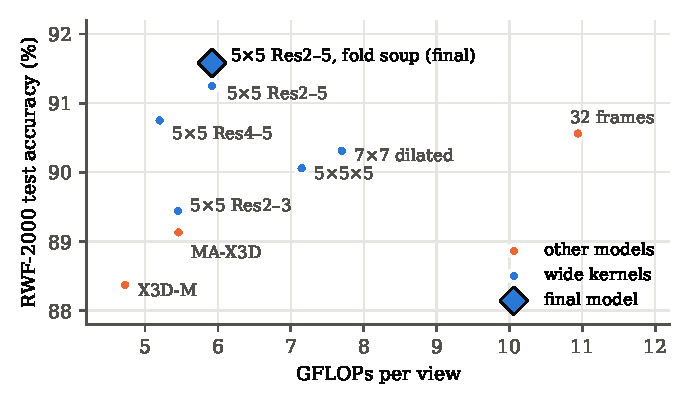
\includegraphics[width=0.78\linewidth]{fig_cost}
\caption{Test accuracy against computation on RWF-2000, uncropped pipeline.
Circles: mean of the four fold models, seed 0. Diamond: the final model,
fold soup, mean of three seeds.}
\label{fig:cost}
\end{figure}

Table~\ref{tab:compare} places the result among published models. The
published numbers are not strictly comparable, since they are obtained on
the official split, which contains the duplicated clips, usually without
stating how the checkpoint was chosen; the selection alone is worth about
0.8 points (Sect.~\ref{sec:protocol-worth}). Under our protocol the model
is the most accurate below 5M parameters and trails a VideoMAE-B
transformer, trained on the same pipeline, by 2.4 points at a twenty-fifth
of its parameters.

\begin{table}[t]
\centering
\caption{RWF-2000 test accuracy. Top: as reported, official split,
selection procedure mostly unstated. Bottom: this paper's protocol.
$^\dagger$Trained on RWF-2000, Hockey Fights and RLVS.}
\label{tab:compare}
\setlength{\tabcolsep}{5pt}
\begin{tabular}{lccc}
\toprule
Method & Params & GFLOPs & Test acc. \\
\midrule
Flow Gated Network~\cite{rwf2000}   & --    & --   & 87.25 \\
SepConvLSTM~\cite{sepconvlstm}      & --    & --   & 89.75 \\
MDCN~\cite{mdcn}                    & $<$1M & --   & 89.70 \\
BiLTMA~\cite{biltma}                & 4.48M & --   & 90.25 \\
VideoMAE~\cite{videomae,mixvit}     & 67--305M & -- & 91.8--92.4 \\
CUE-Net~\cite{cuenet}               & 354M  & $\sim$5800 & 94.00 \\
\midrule
X3D-M, uncropped (3 seeds)          & 2.98M & 4.73 & 88.18 \\
VideoMAE-B, uncropped$^\dagger$     & 86.2M & 135  & 94.00 \\
Ours: $5\times5$ Res2--Res5, fold soup (3 seeds) & 3.27M & 5.92 & \textbf{91.58} \\
\bottomrule
\end{tabular}
\end{table}

\subsection{What the protocol is worth}
\label{sec:protocol-worth}

Two effects outside the model are of the same size as the modules we
tested. Logging test accuracy after every epoch, choosing the epoch by test
accuracy instead of validation F1 inflates the reported number by 0.8
points on average on RWF-2000. And on Hockey Fights, one seed gave the two
modules a significant $+1.25$ OOF points ($p=0.006$) that three seeds
turned into $-0.04$. Under the usual practice, either effect alone could produce a
published improvement.

%======================================================================
\section{Conclusion}

We measured what improves a compact violence detector under a protocol that
removes duplicated clips, keeps same-scene clips together, decides out of
fold and scores each test split once. The largest effect is in the input
pipeline: cropping the video to detected people costs about three points,
and the best pipeline uses no detector. Inside the network, widening the
channel-wise kernels of every stage to $5\times5$ adds 2.63 test points
over three seeds and fuses away at inference, with most of the gain in the
late stages, while a motion-attention gate adds nothing and does not use
its motion input. Averaging the fold models that the protocol trains
anyway gives a single model as accurate as their ensemble. The resulting
detector reaches 91.6\% on RWF-2000 with 3.3M parameters and 5.9 GFLOPs.
Two limitations remain: most comparisons beyond the central one use a
single seed, and the pipeline study covers RWF-2000 only. We release the
splits, the duplicate audit, the rebuilt pipelines and the training code.

\bibliographystyle{splncs04}
\bibliography{refs}

\end{document}
